\section{Einleitung}\label{einleitung}
Moderne Simulationen sind in der Lage grosse Mengen an Daten zu produzieren. Die daraus entstehenden Datenmengen sind oft zu gross um sie zu archivieren oder in vernünftiger Zeit über eine Internetverbindung zu übertragen. In den hier betrachteten wissenschaftlichen Simulationen werden natürliche Phänomene wie Schwingungen, Flugbahnen, Kraftfelder etc. als Menge von Kurven im dreidimensionalen Raum abgebildet. Die Kurven sind dargestellt als Folge von Strecken. Ziel der Arbeit ist es eine verlustbehaftete Kompression für die Folge von Strecken zu entwickeln, welche es ermöglicht solche Daten über eine Internetverbindung effizient zu übertragen und lokal zwischenzuspeichern.

Im Rahmen dieses Projekts werden Magnetfeldlinien der Sonne komprimiert, die über eine Internetverbindung zum JHelioviewer übertragen werden. Der JHelioviewer ist eine Applikation zur Visualisierung von Satellitenmessdaten und Simulationen der Sonne und wird von der ESA und der FHNW entwickelt. Es ist eine Desktop-Applikation, welche zur Laufzeit Mess- und Simulationsdaten von verschiedenen Servern herunterlädt und visualisiert. Die Abbildung \ref{einleitung::feldlinien} zeigt eine Visualisierung der Sonne, die der JHelioviewer erstellt. Es wurden die Feldlinien zusammen mit einer Satellitenmessung der Sonne visualisiert.

\begin{figure}[!htbp]
\center
	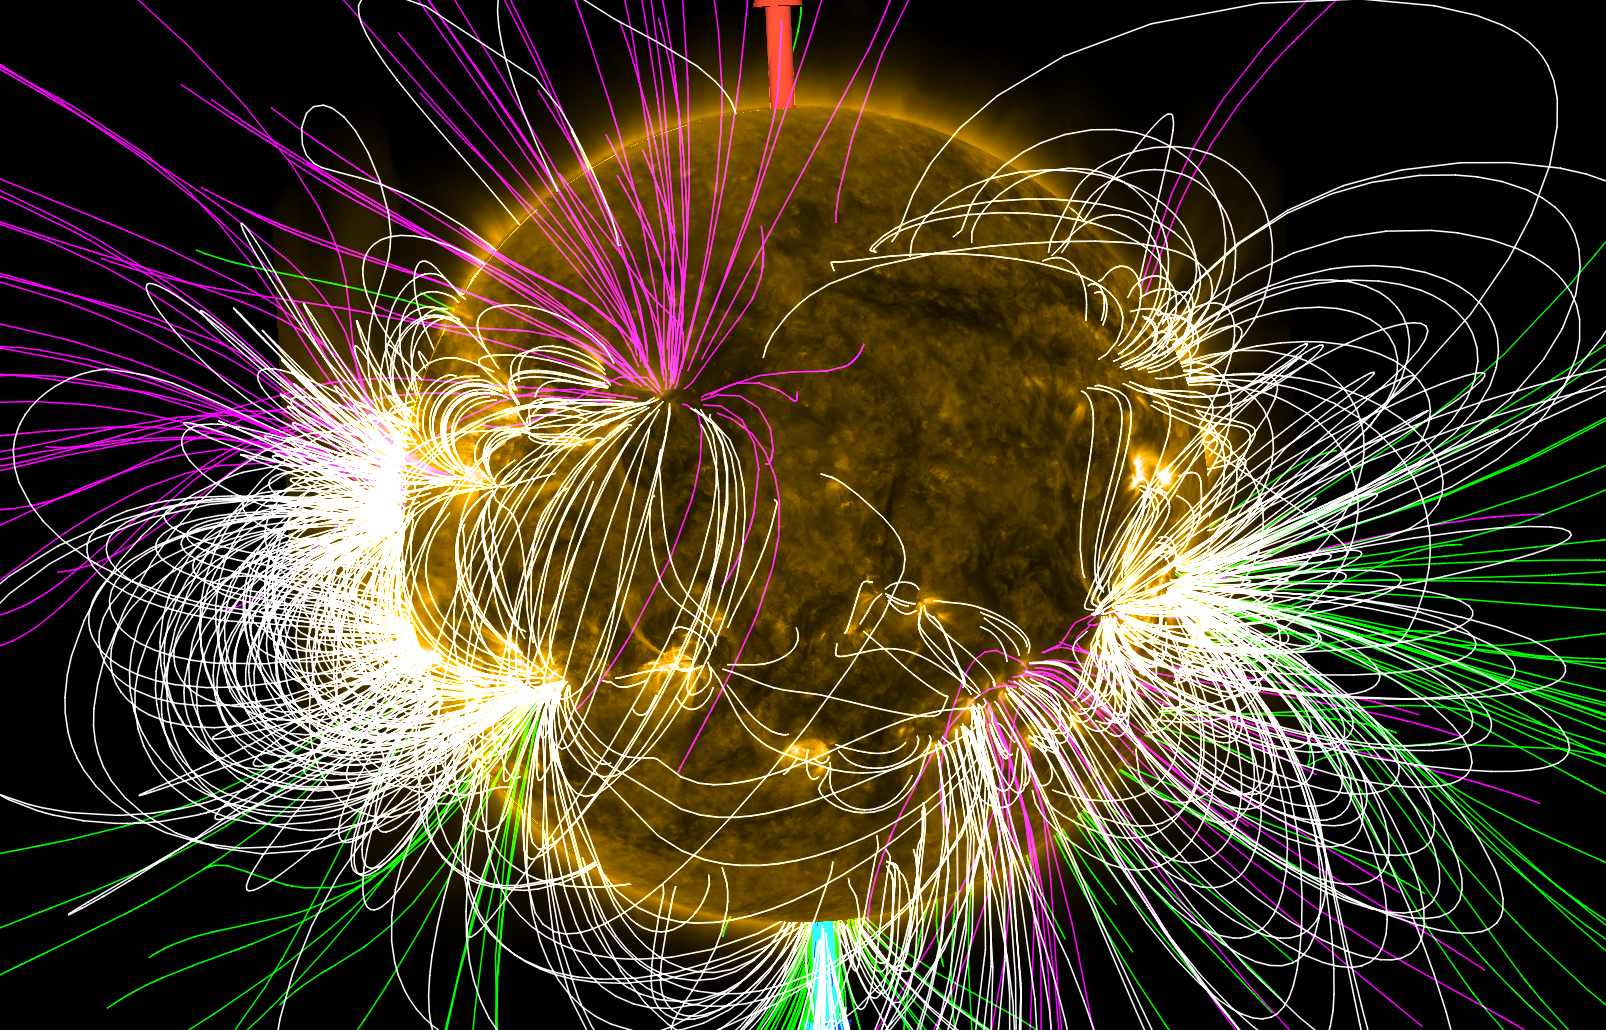
\includegraphics[width=0.8\textwidth,height=8cm,keepaspectratio]{./pictures/einleitung/fieldLines.png}
	\caption{Visualisierung der Feldlinien im JHelioviewer}
	\label{einleitung::feldlinien}
\end{figure}
Auf der Visualisierung sind Feldlinien in drei unterschiedlichen Farben zu erkennen, welche drei unterschiedliche Typen darstellen: Linien, die auf der Sonne starten und auf der Sonne enden, von der Sonne ins Weltall führen oder vom Weltall auf der Sonne enden. Die weissen Feldlinien repräsentieren ''Sonne zu Sonne'', die Grünen ''Sonne ins Weltall'' und die Violetten ''Weltall zur Sonne''.

Der JHelioviewer ist in der Lage eine Abfolge von Mess- und Simulationsdaten als Animation zu visualisieren. Im Anwendungsfall des JHelioviewer werden zwischen 1 und 20 Visualisierungen in der Sekunde angezeigt, wobei 20 die obere Grenze repräsentiert. Die Daten der Animation werden entweder mit einem Streaming kontinuierlich heruntergeladen oder zuvor im Arbeitsspeicher abgelegt. Der JHelioviewer legt maxima Mess- und Simulationsdaten für 1000 Visualisierungen im Arbeitsspeicher ab. Für die Feldlinien wurde eine verlustbehaftete Kompression entwickelt, welche die Datenmenge auf durchschnittlich 1 Megabyte pro Simulation reduziert. Eine Simulation besteht aus einer Menge von etwa 1200 Feldlinien. Für das Caching der Feldliniensimulationen benötigt der Ist-Zustand etwa 1 Gigabyte an Arbeitsspeicher. Der Arbeitsspeicher wird ebenfalls für das Caching von weiteren Mess- und Simulationsdaten benötigt, weshalb diese Datenmenge für die Feldlinien nicht vertretbar ist. Für das Caching wird eine Kompressionsrate zwischen Faktor 8 und 10 benötigt. Zusätzlich wurde erforscht mit welchen Kompromissen das Streaming der Feldlinien möglich ist. Die Animation der Feldlinien wird in einer tieferen Kadenz benötigt. Die obere Grenze liegt bei etwa 10 Feldlinien-Visualisierungen pro Sekunde. Für ein Streaming werden maximal 10 Simulationen in der Sekunde heruntergeladen. Im durchschnittlichen Anwendungsfall werden 1 bis 5 Simulationen pro Sekunde benötigt. Wenn von einer Bandbreite von 5 Megabit für die Feldliniensimulationen angenommen wird, ist mit der Ist-Kompression eine Übertragung von 0.6 Simulationen in der Sekunde möglich. Um unter dieser Bandbreite den durchschnittlichen Anwendungsfall zu ermöglichen, wird ein Kompressionsfaktor von mindestens 10 benötigt. Um den Maximalfall zu ermöglichen ist ein Faktor von 16 nötig.

Im Laufe des Projekts wurden drei Kompressionsverfahren entwickelt. Die Kompressionsraten sind der Tabelle \ref{einleitung:tabelle} ersichtlich. Die Visualisierung der komprimierten Feldlinien kann in den Abbildungen \ref{einleitung:artefakte} verglichen werden. In dieser Arbeit wurde darauf geachtet, dass die Artefakte sich minimal ausprägen und sich die Feldlinien kaum von den Ist-Zustand unterscheiden.
\begin{table}[!htbp]
	\center
	\begin{tabular}{r|l}
		Lösungsansatz & Kompressionsrate \\\hline
		Ohne Kompression & 0.1\\
		Ist-Zustand & 1\\
		Adaptives Subsampling & 11.6 \\
		Diskrete Kosinus Transformation & 14.1 \\
		Prädiktive Kodierung & 13.6\\
	\end{tabular}
	\caption{Kompressionsraten der Lösungsansätze zu einer vergleichbaren Qualität.}
	\label{einleitung:tabelle}
\end{table}
\begin{figure}[!htbp]
\center
\frame{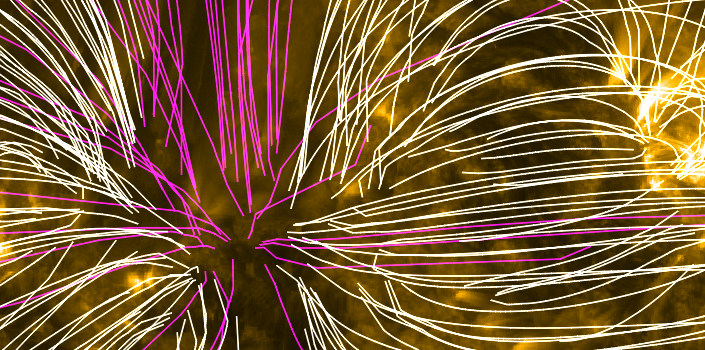
\includegraphics[width=0.49\textwidth,keepaspectratio]{./pictures/einleitung/orig_lines.png}
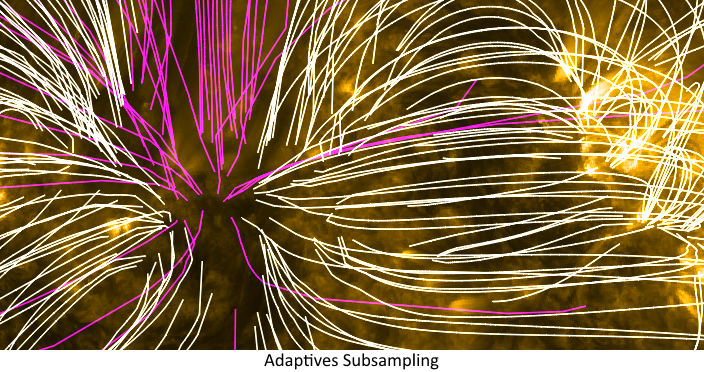
\includegraphics[width=0.49\textwidth,keepaspectratio]{./pictures/einleitung/sol0_lines.png}}
\frame{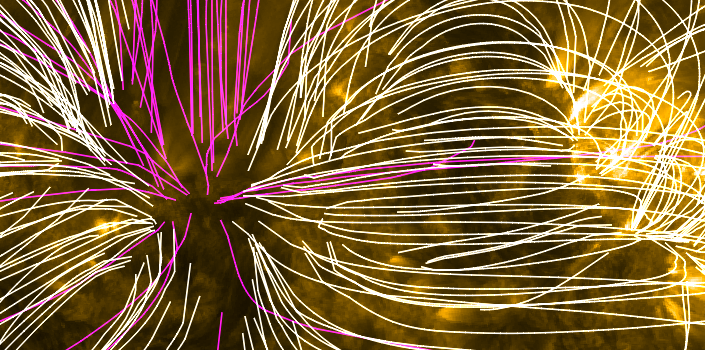
\includegraphics[width=0.49\textwidth,keepaspectratio]{./pictures/einleitung/sol1_lines.png}
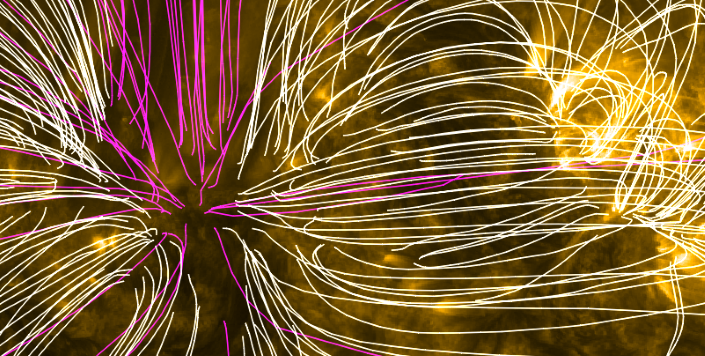
\includegraphics[width=0.49\textwidth,keepaspectratio]{./pictures/einleitung/sol2_lines.png}}
\caption{Dekomprimierte Feldlinien.}
\label{einleitung:artefakte}
\end{figure}
